\subsection{Model Validation}
\label{subsec:model_validation}



\begin{figure}[ht] % Robustness Check
  \centering
  \begin{subfigure}[b]{.49\textwidth}
    \centering
    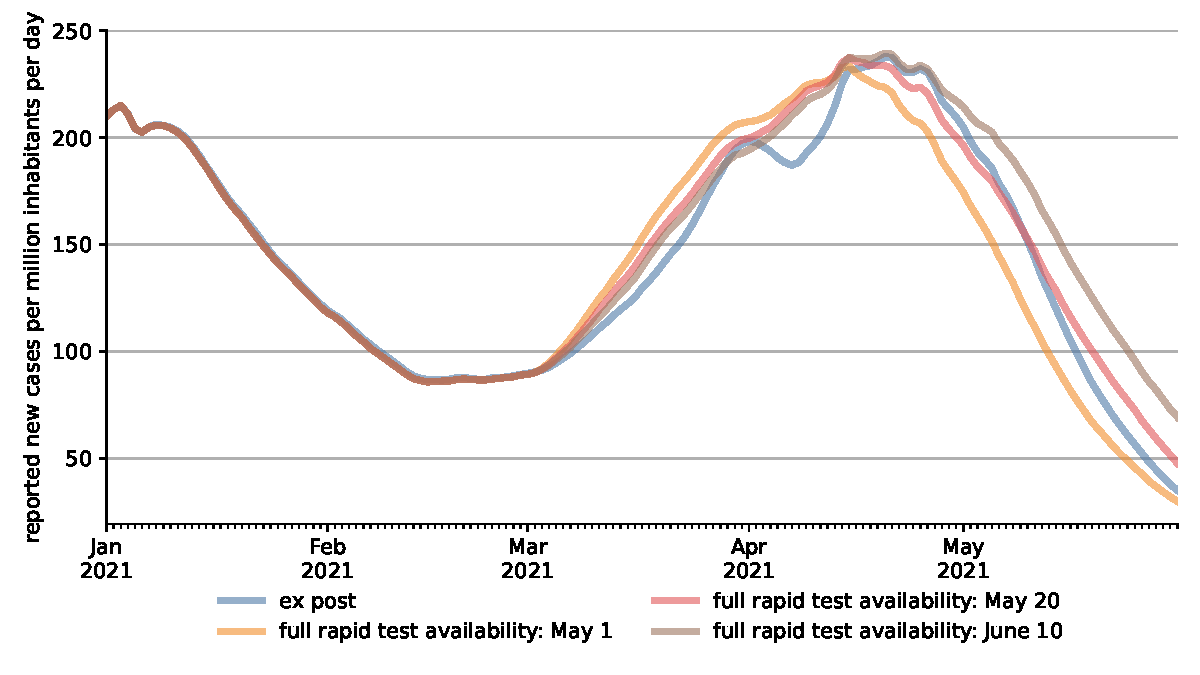
\includegraphics[width=0.9 \textwidth]{figures/results/figures/scenario_comparisons/robustness_check/full_new_known_case}
    \caption{Reported Cases}
    \label{fig:robustness_check_new_known_case}
  \end{subfigure}%
  \hfill
  \begin{subfigure}[b]{.49\textwidth}
    \centering
    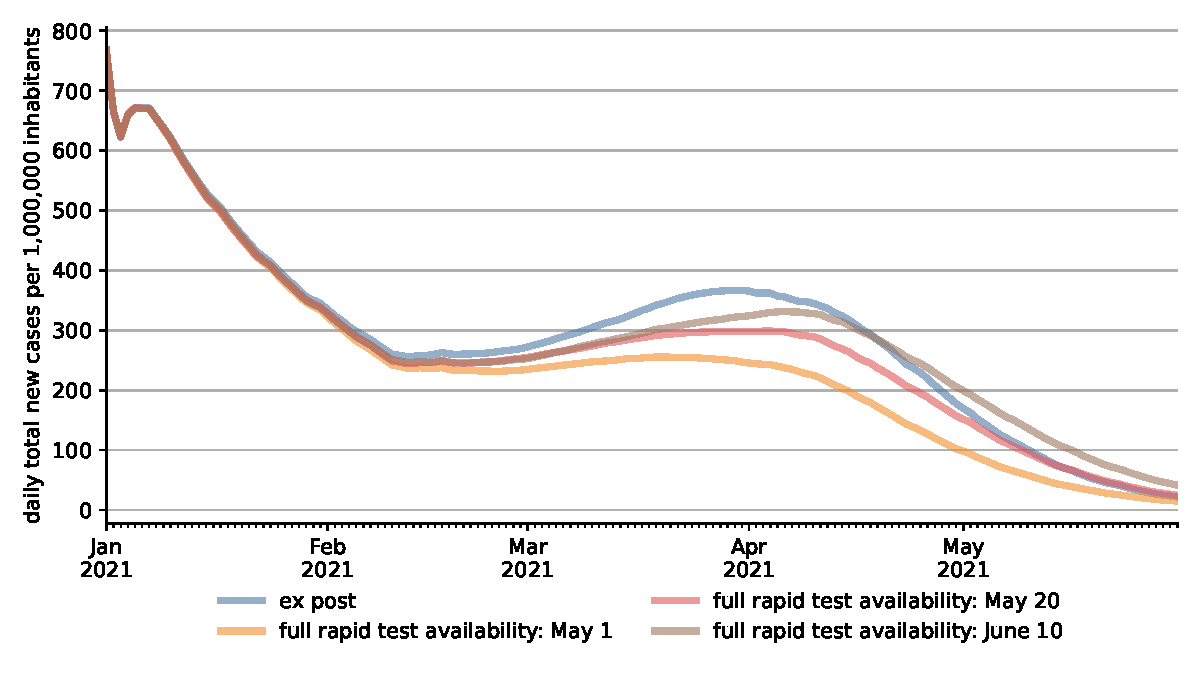
\includegraphics[width=0.9 \textwidth]{figures/results/figures/scenario_comparisons/robustness_check/full_newly_infected}
    \caption{Total Cases}
    \label{fig:robustness_check_newly_infected}
  \end{subfigure}
  \caption{Robustness Check}
  \label{fig:robustness_check_detailed}
  \floatfoot{\noindent \textit{Note:} \textcolor{red}{To be written}}
\end{figure}

 \comment[id=K]{@Janos: Please add caption and description for the robustness check.}
